\chapter{The Random Voting Model: When Chance Explains Choice}
\label{chap5}

In the previous chapter, we uncovered a remarkable universal pattern in electoral statistics: the scaled distribution of the specific margin (margin-to-turnout ratio) follows a consistent curve across diverse democracies, electoral systems, and scales. This universality emerged despite the vast differences in raw turnout and margin distributions across countries. We introduced the Random Voting Model (RVM) as a simple stochastic framework that remarkably captures this universal pattern with surprising accuracy.

Building on this discovery, this chapter provides a comprehensive analysis of the RVM from first principles. We will delve into its mathematical foundations, derive key analytical results, and demonstrate how this elegantly simple stochastic model can explain multiple empirical findings from electoral data. Through both analytical derivations and simulation results, we'll show that the RVM not only predicts the universal specific margin distribution but also connects turnout distributions to margin distributions across different electoral contexts.

\section{Introducing the Random Voting Model (RVM): Simplicity by Design}
\label{sec:RVM_intro}
The Random Voting Model is based on the premise that electoral outcomes can be understood through a minimal statistical framework that captures the essence of competition without modeling voter psychology or strategic behavior. The model is parameter-free beyond the turnout distribution and number of candidates, relying only on simple probabilistic principles.

In this Random Voting Model, $c_i$ number of candidates contest at $i$-th electoral unit with $n_i$ electors (voters) and each elector from the $i$-th electoral unit casts their vote for $j$-th candidate with a probability $p_{ij}$. These probabilities are assigned as follows: for each candidate, a number between $0$ and $1$ is drawn uniformly at random, which is assigned as an unnormalized probability weight $w_{ij}$ to that candidate. The weights are subsequently normalized to get the probability $p_{ij}, j = 1, 2 \dots c_i$ of receiving the vote of an elector. This can be mathematically stated as
\begin{equation}
    w_{ij} \sim \mathcal{U}(0, 1) \quad \text{and} \quad p_{ij} = \frac{w_{ij}}{\sum_k w_{ik}}, \text{ with } j = 1, 2 \dots c_i,
    \label{eq:RVM_prob}
\end{equation}
where $\mathcal{U}(0, 1)$ denotes a uniformly distributed random variable in $(0,1)$.

After each of the $n_i$ electors (voters) in $i$-th electoral unit casts their vote for some candidate $j$ independently with probability $p_{ij}$, the candidate receiving the most votes $V_{i, w}$ is declared the winner, and the candidate securing the next largest number of votes $V_{i, r}$ is the runner-up. The \emph{margin of victory} $M_i$ is then defined to be the vote difference between the winner and the runner-up: \emph{i.e.} $M_i = V_{i, w} - V_{i, r}$. The empirical election data we employ shows that the top three candidates, on average, account for nearly 87\% of all votes polled in an election.
Hence, as part of the model specification, we fix the number of candidates in each electoral unit to be three, i.e., $c_i = 3$ for all $i$.

The only input to this model is the raw turnout data, i.e., the number of voters (who actually voted) in each constituency. For the model simulation, we use the turnout data of real elections as the total number of voters in different constituencies. To understand how simulations are performed, consider this notional example: if a country has $N=100$ constituencies and data for five such elections is available. Then, the model is simulated on $500$ electoral units. The number of electors in each electoral unit is taken from the consolidated turnouts. Such a simulation of election is performed multiple times to get the average distributions.
\section{The RVM's First Symphony: Obtaining the Universal $Q_{\widetilde{\mu}}\left(\widetilde{\mu}\right)$}
\label{sec:RVM_first_symphony}
We now demonstrate how the RVM explains the universal distribution of scaled specific margin $Q_{\widetilde{\mu}}\left(\widetilde{\mu}\right)$ observed in the previous chapter. As mentioned in the previous section (\ref{sec:RVM_intro}), we consider the case where $3$ candidates are contesting in an election. The weight assigned for the $j$-th candidate of the $i$-th electoral unit is $w_{ij}$. These weights are drawn independently at random from a uniform distribution between $0$ and $1$.  The corresponding probability $p_{ij}$ of receiving votes is calculated by normalizing these weights. Hence, we have the following,
\begin{equation}
    w_{ij} \sim \mathcal{U}(0, 1) \text{ and } p_{ij} = \frac{w_{ij}}{\sum_{k=1}^3 w_{ik}}; \text{ with } j = 1, 2, 3.
\end{equation}
For the rest of the analysis in this chapter, we focus on a single ($i$-th) electoral unit with voter turnout $T$ and drop the corresponding index $i$ for brevity. Hence,
\mathtoolsset{centercolon}
\begin{equation}
    w_{ij} := w_j \text{ and } p_{ij} := p_j.
\end{equation}
\subsection{The Set-up: Large Turnout Limit}
For large turnout $(T \gg 1)$, it is reasonable to assume the number of votes received by $j$-th candidate is proportional to their probability $p_j$, in particular, $v_j \approx p_j T$. Hence, for $T \gg 1$, the \emph{margin} can be approximated as 
\begin{equation}
M \approx (p_{max} - p_{2nd \: max})T,
\end{equation}
where $p_{max}$ and $p_{2nd \:max}$ correspond to the largest and the second largest probabilities assigned to the candidates. For example, if the probabilities $p_1, p_2,$ and $p_3$ assigned to the 3 candidates are $0.1, 0.6,$ and $0.3$, then $p_{max} = p_2 = 0.6$ and $p_{2nd \:max} = p_3 = 0.3$. The margin $M$ can also be written in terms of $w_j$ as the following:
\begin{center}
\begin{align}
    \nonumber M &\approx \left(\frac{w_{max}}{w_1 + w_2 + w_3} - \frac{w_{2nd\:max}}{w_1 + w_2 + w_3}\right)T,\\
    \nonumber & = \left(\frac{w_{(3)}}{w_{(1)} + w_{(2)} + w_{(3)}} - \frac{w_{(2)}}{w_{(1)} + w_{(2)} + w_{(3)}}\right)T,\\
    & = \left(\frac{w_{(3)} - w_{(2)}}{w_{(1)} + w_{(2)} + w_{(3)}}\right)T,
\end{align}

\end{center}
where $w_{(k)}$ is the $k$-th order statistics \cite{BarBalNag2008}. Hence, 
\begin{center}
\begin{align}
    \frac{M}{T} \approx \frac{w_{(3)} - w_{(2)}}{w_{(1)} + w_{(2)} + w_{(3)}}.
    \label{eq:S6}
\end{align}
\end{center}
\subsection{Order Statistics: The Key to Understand Ranking}
Consider $n$ \emph{iid} random variables $\{X_1, X_2 \dots X_n\}$ drawn from a distribution $\rho(x)$. When arranged in ascending order, the random variable at the $k$-th spot is defined as the $k$-th order statistics. In particular, $n$-th and $1$-st order statistics correspond to the maximum and minimum of those $n$ random variables, respectively. The $k$-th order statistics of the random variable $X$ is denoted by $X_{(k)}$.

The joint probability density of all the order statistics of the above-mentioned $n$ random variables, $\mathbbm{P}\left(x_{(1)}, x_{(2)}, ... x_{(n)}\right)$, defined as the probability density that the random variable $X_{(k)}$ takes the value $x_{(k)}$ for $k \in \{ 1, 2, \dots, n\}$, is
\begin{equation}
    \mathbbm{P}\left(x_{(1)}, x_{(2)}, ... x_{(n)}\right) = n!\prod_{k=1}^{n}\rho\left(x_{(n)}\right).
\end{equation}
\subsection{Back to Reality: RVM's First Symphony}
Now that we understand the joint probability density of the order statistics, for RVM, we have $n = 3$ and $\rho(x) = \mathcal{U}(0, 1)$. Hence we have,    
\begin{center}
    \begin{align}
        \mathbbm{P}\left(w_{(1)}, w_{(2)}, w_{(3)}\right) = 3! = 6; \text{ with } 0<w_{(1)}<w_{(2)}<w_{(3)}<1,
    \end{align}
\end{center}
and $\mathbbm{P}\left(w_{(1)}, w_{(2)}, w_{(3)}\right) = 0$ otherwise, with the following normalization:
\begin{equation}
    \int_{0}^{1}dw_{(3)}\int_{0}^{w_{(3)}}dw_{(2)}\int_{0}^{w_{(2)}} 6 dw_{(1)} = 1.
\end{equation}
From the joint probability distribution of all the order statistics, we calculate the approximate probability density function of specific margin $ M / T = \mu$ from Eq.~\eqref{eq:S6} as follows, 
\begin{center}
    \begin{align}
        \nonumber Q_{\mu}\left(\mu\right) & = 6 \nonumber \int_{0}^{1}dw_{(3)}\int_{0}^{w_{(3)}}dw_{(2)}\int_{0}^{w_{(2)}} \delta\left(\mu - \frac{w_{(3)}- w_{(2)}}{w_{(1)} + w_{(2)} + w_{(3)}}\right)dw_{(1)},\\
        & = 6 \int_{0}^{1}dw_{(3)}\int_{0}^{w_{(3)}} \frac{w_{(3)} - w_{(2)}}{\mu^2} \nonumber \mathbbm{1}_{0<\frac{w_{(3)} - \mu w_{(3)} - (1 + \mu)w_{(2)}}{\mu}<w_{(2)}} dw_{(2)},\\
        & = 6 \int_{0}^{1}dw_{(3)} \frac{(1 - \mu)(5 + 7\mu)w_{(3)}^2}{2(1 + \mu)^2(1 + 2\mu)^2}.\\
    \end{align}
\end{center}
Finally, after performing this integral, we get 
\begin{equation}
    Q_{\mu}\left(\mu\right) = \frac{(1 - \mu)(5 + 7\mu)}{(1 + \mu)^2(1 + 2\mu)^2}.
\end{equation}
The distribution $Q_{\mu}\left(\mu\right)$ does not depend on the turnout and is universal. Now, by a change of variable to scaled specific margin defined as $\widetilde{\mu} = \mu / \langle \mu \rangle$, we obtain its distribution $Q_{\widetilde{\mu}}\left(\widetilde{\mu}\right)$ to be
\begin{equation}
    Q_{\widetilde{\mu}}\left(\widetilde{\mu}\right) = \langle \mu \rangle ~ Q_{\mu}\left( \widetilde{\mu} \langle \mu \rangle \right) =  \frac{\langle \mu \rangle(1 - \widetilde{\mu} \langle \mu \rangle)(5 + 7\widetilde{\mu} \langle \mu \rangle)}{(1 + \widetilde{\mu} \langle \mu \rangle)^2(1 + 2\widetilde{\mu} \langle \mu \rangle)^2}, 
\end{equation}
where $\langle \mu\rangle = \frac{1}{2}+\ln \left(\frac{9 \sqrt[4]{3}}{16}\right)$.
This derived distribution $Q_{\widetilde{\mu}}\left(\widetilde{\mu}\right)$ is precisely the universal curve observed in the empirical data across 32 countries in the previous chapter. The remarkable agreement between theory and data as shown in Fig.~\ref{fig:RVM_mu} confirms that the RVM captures the essential statistical features underlying electoral competition.

\begin{figure}[H]
    \centering
    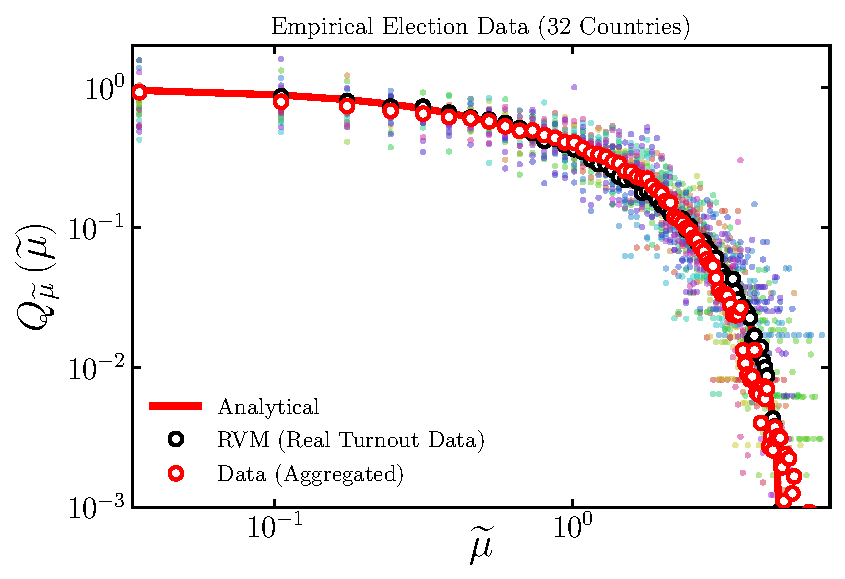
\includegraphics[width=0.95\textwidth]{chapters/chapter5/universality_empirical_analytical.pdf}
    \caption{$Q_{\widetilde{\mu}}\left(\widetilde{\mu}\right)$: The distribution is universal and does not depend on the turnout distribution. Each color indicates empirical $Q_{\widetilde{\mu}}\left(\widetilde{\mu}\right)$ for a specific country for which the election data is consolidated over several elections. The average of these empirical distributions (red open circles) closely follows the analytical curve (red line) and the averaged RVM predictions for each country (black open circles).}
    \label{fig:RVM_mu}
\end{figure}

\section{Expanding the Repertoire: Predicting Margins from Turnouts}
Having established that the RVM predicts the universal specific margin distribution, we now explore how the model can predict the margin distribution $Q_M(M)$ from an arbitrary turnout distribution $g(T)$. From the previous section, we have the distribution of the specific margin $\mu = M / T$ to be
\begin{equation}
    Q_{\mu}\left(\mu\right) = \frac{(1 - \mu)(5 + 7\mu)}{(1 + \mu)^2(1 + 2\mu)^2}.
\end{equation}
Through a simple change of variable $(M = \mu T)$ we get,
\begin{equation}
    \mathcal{P}(M|T) = \frac{(1 - M / T)(5 + 7M /T)}{T(1 + M / T)^2(1 + 2M / T)^2}.
\end{equation}
For an arbitrary turnout distribution $g(T)$, we obtain the distribution of $M$ to be,
\begin{equation}
    Q_M(M) = \int_{M}^{\infty}g(T)\mathcal{P}(M |T) dT = \int_{M}^{\infty}g(T)\frac{(1 - M / T)(5 + 7M /T)}{T(1 + M / T)^2(1 + 2M / T)^2} dT.
\end{equation}
Again with $u = T / M$, the above integral transforms to,
\begin{equation}
    Q_M(M) = \int_{1}^{\infty}g(Mu)\frac{u(u - 1)(5u + 7)}{(1 + u)^2 (2 + u)^2}du.
    \label{eq:pm}
\end{equation}
\subsection{Turnout Distribution Effects on Margin Distribution}
We compute $Q_M(M)$ for different turnout distributions $g(T)$. In particular, we take $g(T)$ to be (A) exponential, (B) power law, and (C) Gaussian distributions as they have vastly different tail behaviors. Finally we also consider a uniform turnout distribution with finite support.
\subsubsection{Exponential Turnout Distribution}
In this case $g(T) = \frac{1}{\tau}e^{-T / \tau}$, with $ \tau> 0$. Hence,
\begin{equation}
    Q_M(M) = \int_{1}^{\infty}\frac{1}{\tau}e^{-Mu / \tau} \frac{u(u - 1)(5u + 7)}{(1 + u)^2 (2 + u)^2}du,
\end{equation}
or,
\begin{equation}
    Q_M(M) = \frac{e^{-\frac{M}{\tau}}}{\tau^2} \left(4 e^{\frac{2 M}{\tau}} (\tau+M) \text{Ei}\left(-\frac{2 M}{\tau}\right)-9 e^{\frac{3 M}{\tau}} (\tau+2 M) \text{Ei}\left(-\frac{3 M}{\tau}\right)-4 \tau\right), 
\end{equation}
where $\text{Ei}(x) = \int_{-\infty}^{x}\frac{e^t}{t}dt$. At large margin limit $(M \rightarrow \infty)$, the asymptotic behavior of the distribution is the following (up to the leading order of $M$):
\begin{equation}
    Q_M(M)= \frac{\tau}{3M^2}e^{-M/\tau}.
\end{equation}
This suggests that in the large margin limit, both the margin and its corresponding turnout distribution have an exponential decay with the same rate.
\subsubsection{Power law Turnout Distribution}
In this case $g(T) = \frac{\alpha - 1}{T_{min} ^{1 -\alpha}} T ^ {-\alpha}$, with $\alpha > 1$ and $T>T_{min}$. Hence we have,
\begin{equation}
    Q_M(M) = \int_{1}^{\infty}\frac{\alpha - 1}{T_{min} ^{1 -\alpha}} (Mu) ^ {-\alpha} \frac{u(u - 1)(5u + 7)}{(1 + u)^2 (2 + u)^2}du,
\end{equation}
or,
\begin{equation}
    Q_M(M) = C(M)\frac{\alpha - 1}{T_{min} ^{1 -\alpha}} (M) ^ {-\alpha}, 
    \label{eq:powerlaw}
\end{equation}
where,
\begin{numcases}{C(M) = }
    I_1(\infty) - I_1(T_{min} / M) , \text{if } M\leq T_{min}\\
    I_1(\infty) - I_1(1), \text{otherwise,}
\end{numcases}
with,
\begin{equation}
    I_1(y) = \int \frac{y^{1 - \alpha}(y - 1)(5y + 7)}{(1 + y)^2 (2 + y)^2}dy,
\end{equation}
and,
\begin{numcases}{I_1(y)=}
     -\frac{4}{y+1}+\frac{9}{2 (y+2)}-\frac{1}{4} 7 \ln (y)+4 \ln (y+1)-\frac{9}{4} \ln (y+2), \text{if } \alpha = 2 \\
     \frac{y^{2-\alpha } \left(16 \, _2F_1(2,2-\alpha ;3-\alpha ;-y)-9 \, _2F_1\left(2,2-\alpha ;3-\alpha ;-\frac{y}{2}\right)\right)}{4 (\alpha -2)}, \text{otherwise,} \\
\end{numcases}
where ${}_{2}F_{1}(a,b;c;z)$ is a hypergeometric function \cite{abramowitz_stegun}, defined as,
\begin{align*}
    {\displaystyle {}_{2}F_{1}(a,b;c;z)  =\sum _{n=0}^{\infty }{\frac {(a)_{n}(b)_{n}}{(c)_{n}}}{\frac {z^{n}}{n!}}=1+{\frac {ab}{c}}{\frac {z}{1!}}+{\frac {a(a+1)b(b+1)}{c(c+1)}}{\frac {z^{2}}{2!}}+\cdots .}\\
\end{align*}

It is evident from Eq.~\eqref{eq:powerlaw} that for $M > T_{min}$, the margin distribution decays with a power law exponent $\alpha$, exactly the same as the turnout distribution.
\subsubsection{Gaussian Turnout Distribution}
In this case $g(T) = C_0 e^{-(T/T_0)^2}$, with $T>0$. Hence,
\begin{equation}
     Q_M(M) = \int_{1}^{\infty} C_0 e^{-(Mu/T_0)^2}\frac{u(u - 1)(5u + 7)}{(1 + u)^2 (2 + u)^2}du.
\end{equation}
At large margin limit $(M \rightarrow \infty)$, the asymptotic behavior of the distribution is the following (up to the leading order of $M$):
\begin{equation}
    Q_M(M) = \frac{C_0}{12}\left(\frac{T_0}{M}\right)^4 e^{-\left(M/ T_0\right)^2}, 
\end{equation}
and it has a Gaussian decay similar to the corresponding turnout distribution.\\

From the asymptotic analysis of the margin distributions for the three above-mentioned turnout distributions, we provide strong evidence that the tails of the margin distributions mimic that of the corresponding turnout distribution. For completeness, we also compute the margin distribution corresponding to a uniform turnout distribution which has a finite support (no tail behavior).
\subsubsection{Uniform Turnout Distribution}
In this case $g(T) = \frac{1}{b - a}$, when $T \in [a, b]$, otherwise  $g(T) = 0$. Hence,
\begin{numcases}{Q_M(M)= }
    \frac{1}{b - a}\int_{a/M}^{b/M}\frac{u(u - 1)(5u + 7)}{(1 + u)^2 (2 + u)^2}du , \text{if } M\leq a\\
    \frac{1}{b - a}\int_{1}^{b/M}\frac{u(u - 1)(5u + 7)}{(1 + u)^2 (2 + u)^2}du, \text{otherwise,}
\end{numcases}
or, 
\begin{numcases}{Q_M(M)= }
    \frac{1}{b - a} \left(I_2(b / M) - I_2(a / M)\right), \text{if } M\leq a\\
    \frac{1}{b - a}\left(I_2(b / M) - I_2(1)\right),  \text{if } a > M \geq b\\
    0,  \text{ otherwise,}
\end{numcases}
where, 
\begin{equation}
    I_2(y) = \int \frac{y(y - 1)(5y + 7)}{(1 + y)^2 (2 + y)^2}dy = -\frac{4}{y+1}+\frac{18}{y+2}-4 \ln (y+1)+9 \ln (y+2).
\end{equation}
\subsection{RVM Simulations with Synthetic Turnout Distributions}
The RVM enables us to estimate the scaled margin distribution $f(M / \langle M \rangle)$ using only the raw turnout data, indicating that $f(M / \langle M \rangle)$ is driven by the details of the turnout distribution $g(T)$. To further quantify the effect of $g(T)$ on the scaled margin distribution $f(M / \langle M \rangle)$, we simulate elections using RVM, with turnouts drawn from vastly different synthetically generated distributions. In particular, to study the tail behaviors, we use the following four different turnout distributions:
\begin{enumerate}
    \item \textbf{Gaussian Turnout Distribution:} $g(T) = \frac{1}{\sigma\sqrt{2\pi}}\exp\left(-\frac{(T - \mu)^2}{2\sigma^2}\right), \text{ with } \mu = 50000$, $\sigma = 10000$ and $T > 0$.
    \item \textbf{Exponential Turnout Distribution:} $g(T) = \frac{1}{\tau} \exp{\left(-\frac{T}{\tau}\right)}, \text{ with } \tau = 50000$.
    \item \textbf{Power law Turnout Distribution:} $g(T) = \frac{\alpha - 1}{T_{min} ^{1 -\alpha}} T ^ {-\alpha}$, with $\alpha = 2$ and $T_{min} = 100$ (minimum possible turnout).
    \item \textbf{Uniform Turnout Distribution:} $T \sim \mathcal{U} (a, b)$, with $a = 100$ and $b = 100000$. $\mathcal{U}(a, b)$ denotes uniform distribution between the range $a$ and $b$.
\end{enumerate}

Each of the RVM simulations was performed on $10^6$ electoral units, with turnouts (rounded down to the nearest integer) drawn from one of these three distributions. The simulation demonstrates that the tail of the margin distribution mimics the turnout distribution's tail.  This is evident in Fig.~\ref{fig_sup_1}(a), (b), and (c). The tail of the margin distribution (Fig.~\ref{fig_sup_1} (c)) corresponding to power law turnouts decays with the same power law exponent.  In the simulation with Gaussian turnout distribution, we find the tail of the margin distribution also has a Gaussian falloff (Fig.~\ref{fig_sup_1} (a)). Similarly, the margin distribution corresponding to exponential turnouts has an exponential tail (Fig.~\ref{fig_sup_1} (b)). As the probability density function of uniform turnout distribution and corresponding margin distribution have finite supports, their tails can not be properly defined. We find a sharp cutoff in the corresponding margin distribution. The analytical (semi-analytical for Gaussian turnout) predictions for the margin distributions (shown as black lines in Fig.~\ref{fig_sup_1}) corresponding to all four aforementioned turnout distributions are in excellent agreement with the RVM simulation. In empirical county-level election data of the United States, the heavy-tailed decay of the turnout distribution is reflected in the corresponding margin distribution (Fig.~\ref{fig_sup_1}(e)). In Fig.~\ref{fig_sup_1} (f), we see a similar decay trend in both margin and turnout distribution, which correspond to congressional district-level election data of the USA. We obtain the scaled margin distribution $f(M / \langle M \rangle)$ by scaling $Q(M)$ by its mean; hence, both $Q(M)$ and $f(M / \langle M \rangle)$ have similar decay and are strongly related to the corresponding turnout distribution $g(T)$.
\begin{figure}[H]
    \centering
    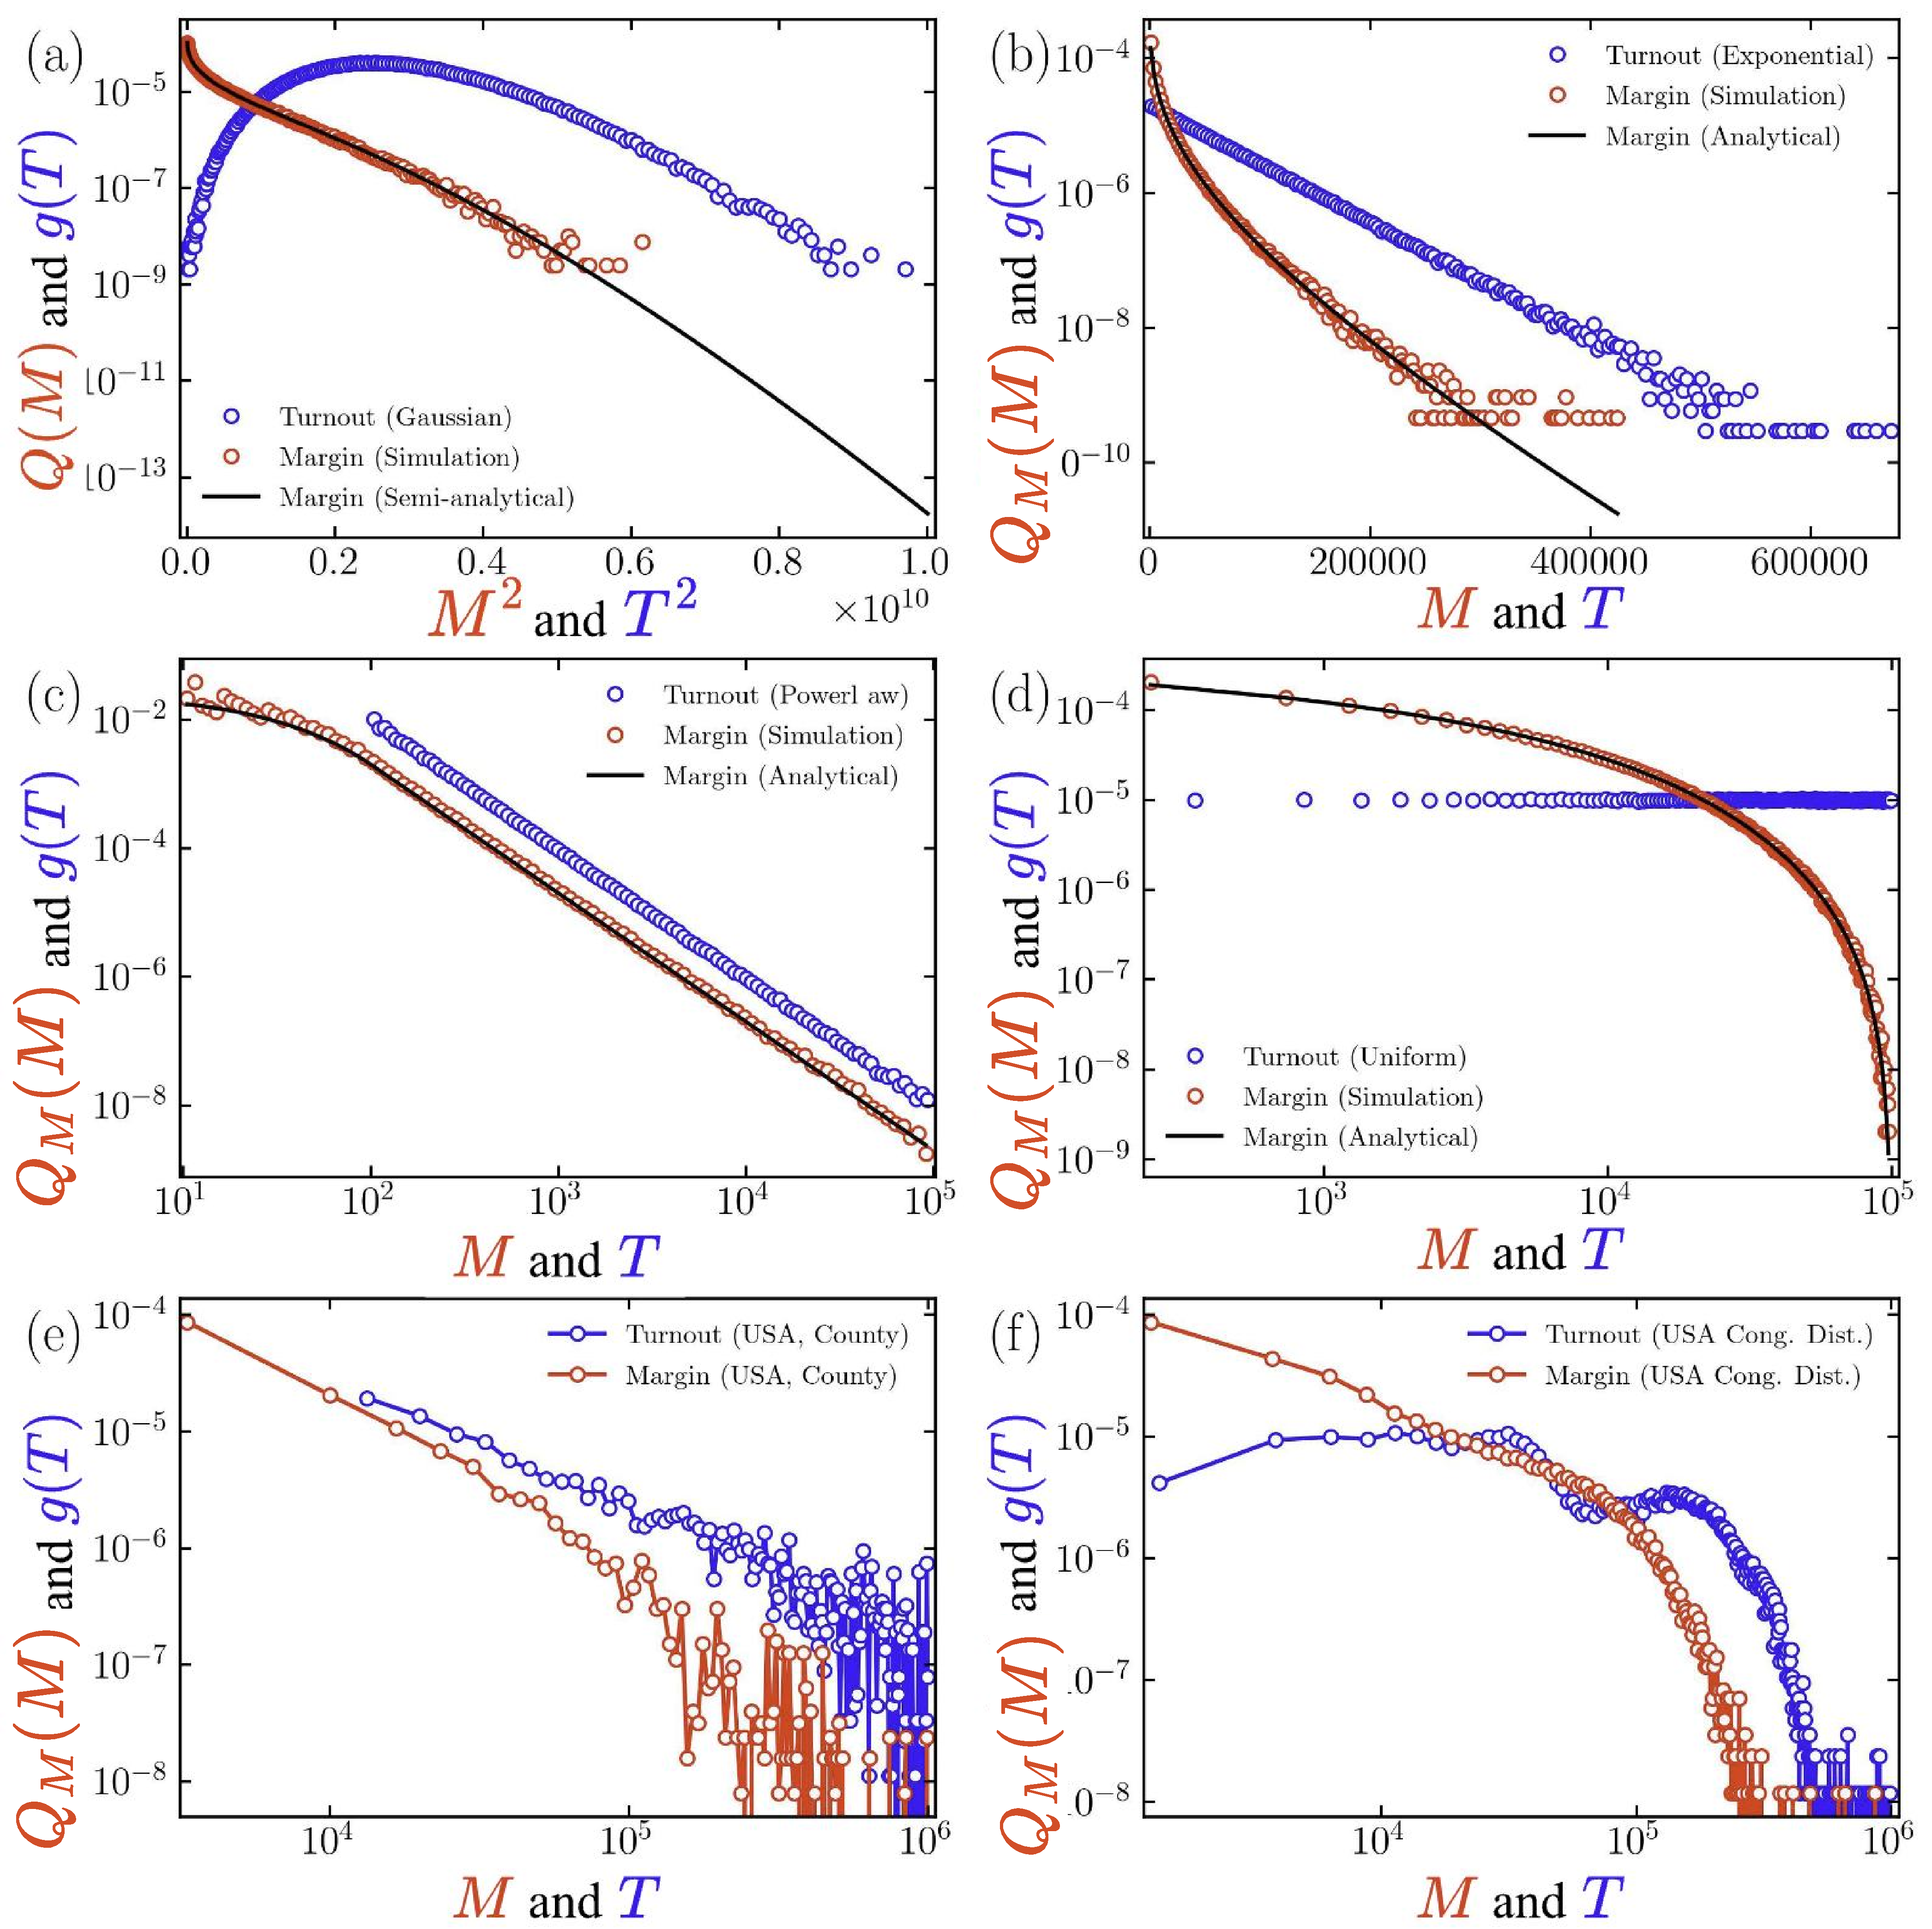
\includegraphics[width=\textwidth]{chapters/chapter5/margin_turnout_dists.pdf}
    \caption{The margin distribution $Q(M)$ is plotted with the corresponding turnout distribution $g(T)$ to demonstrate that the tails of both these distributions are correlated. Panels (a), (b), (c), and (d) correspond to Gaussian, exponential, power law, and uniform turnout distributions, respectively. Blue open circles denote the turnout distributions. Red open circles denote the margin distribution computed through RVM simulations. Black solid lines correspond to the margin distribution computed using Eq.~\ref{eq:pm}. For exponential, power law, and uniform turnout distributions, the integration was analytically calculated, and for Gaussian turnout distribution, it was evaluated numerically. Panels (e) and (f) depict the margin and turnout distribution for the county-level and congressional district-level election data of the USA, respectively.}
    \label{fig_sup_1}
\end{figure}
\subsection{Need of the Hour: Scaling by Mean}
RVM can remarkably predict the overall trend, especially the tail behaviors of the margin distributions $Q_M(M)$. However, the prediction of the whole distribution is sadly not possible, due to RVM's inability of relaiably prediting the mean margin. To surcumnavigate this limitaion, we scale the margin distributions with their sample mean, 

\subsubsection{PC}
% paraphrase
Figure \ref{fig_1}(a) displays the distribution of raw turnout $g(T)$ at the constituency level for national elections in six countries, namely, India, USA, South Korea, Canada, Japan, and Germany. Striking dissimilarities in $g(T)$ are visible in the shape and support of distribution for countries. For Germany, $g(T)$ has a unimodal character, while that for Canada and the USA display multiple peaks. The corresponding scaled margin $M/\langle M \rangle$ is displayed as distribution $f(M/\langle M \rangle)$ (computed from the consolidated margin data for each country) in Fig.~\ref{fig_1}(b-g). While they appear to be broadly similar, certain differences are clearly noticeable. In particular, $f(M/\langle M \rangle)$ for German elections in Fig.~\ref{fig_1}(g) has a sharp cutoff, but for India and Japan in Fig.~\ref{fig_1}(b, f) the distribution has a slower decay. These observations motivate the questions of whether $f(M/\langle M \rangle)$ is related to the raw turnout distribution and can be obtained from it.

To investigate this question, we propose a Random Voting Model (RVM) ${\mathcal V}(T)$ that takes raw turnouts $T=\{T_1, T_2 \dots T_N\}$ as input. This model emulates an election taking place at $N$ electoral units (say, constituencies). At $i$-th unit, each of the $T_i$ voters (raw turnout at $i$-th unit) can cast only one vote, independently and by randomly choosing one of the $c_i$ contesting candidates. The probability that candidate $j$ in $i$-th unit can attract a vote is $p_{ij}= w_{ij}/\sum_k w_{ik}$, where $w_{ij} \in [0,1]$ is a random number drawn from a uniform distribution. While this protocol provides a natural and effective choice for $p_{ij}$, the sensitivity of the RVM predictions on different protocols is discussed in Sec.~S5 of Ref. \cite{supp}. In election data that we use, averaged over all the 34 countries, the top two (three) candidates account for 79\% (87\%) of all votes polled. Hence, the model assumes three candidates at every constituency: $c_i=3$ for $i=1,2 \dots N$, and that all eligible voters cast their votes, implying $T_i = n_i$. By simulating this model, margin $M_i$ is obtained for $i$-th electoral unit and $\langle M \rangle = (1/N) \sum_{i=1}^N M_i$ is the associated sample mean. For a detailed description of the model, see Sec.~S1 of Ref. \cite{supp}. 

The model predictions depend exclusively on the actual turnout distribution, and no free parameters to be tuned. As illustrated in Fig.~\ref{fig_1}(b - g), the scaled margin distributions predicted by this model (solid lines) show a remarkable agreement with those computed from empirical margin data from real elections. Notably, RVM faithfully captures disparate decay features in  $f(M/\langle M \rangle)$ for India, USA, South Korea, Canada, Japan, and Germany (for 28 other countries, see Sec.~S7 of Ref. \cite{supp}). This suggests that the raw turnout data carries intrinsic information about the margin distribution. RVM effectively leverages this information embedded in the turnout distribution to predict the scaled margin distribution. 
\begin{figure}
    
\end{figure}
\subsubsection{Different Scale}
Next, we show that these results are independent of the number of voters or size of electoral units. In large countries, depending on the size of the electoral unit, the typical turnout can differ by several orders of magnitude. For example, in India, polling booths have a typical electoral size $\sim 10^3$, whereas, at the parliamentary constituency level, it is about $10^6$. Further, the shapes of $g(T)$ are also vastly different at different scales. Figure \ref{fig_2}$(a)$ captures the striking differences in range and shape of $g(T)$ for India, the US, and Canada at two different scales. Quite remarkably, despite these vast differences in the scale, the same RVM ${\mathcal V}(T)$, without any parameter adjustments, accurately predicts the scaled margin distribution. Figure \ref{fig_2}$(b, c, d)$ shows the empirical distribution of scaled margins (in national elections) at the constituency-level scale, and Figure \ref{fig_2}$(e, f, g)$ shows the same at the scale of polling booths (county for USA).

\begin{figure}
    
\end{figure}

\subsubsection{All 32 Countries}
Further in figure X we demonstrate the remarkable prediction scaled margin distributions by RVM.

\begin{figure}
    
\end{figure}

\section{Conclusion: The Power and Limitations of RVM}

In this chapter, we have provided a comprehensive analysis of the Random Voting Model (RVM) from its first principles. We demonstrated how this elegantly simple model generates the universal distribution of scaled specific margins observed across diverse electoral systems worldwide. Through rigorous mathematical derivations, we showed that the model successfully predicts this universality without requiring any parameters beyond the turnout distribution and number of candidates.

Furthermore, we established that the RVM provides powerful insights into how turnout distributions shape margin distributions across different electoral contexts. Through both analytical solutions and simulations with various synthetic turnout distributions (Gaussian, exponential, power law, and uniform), we demonstrated that margin distributions inherit the tail behavior of their corresponding turnout distributions. This finding explains why electoral margin distributions can vary dramatically across countries while still adhering to the universal specific margin pattern.

The model's ability to predict scaled margin distributions from raw turnout data alone—without any adjustments or free parameters—is remarkable and represents a significant advance in our understanding of electoral statistics. It suggests that beneath the apparent complexity and diversity of electoral systems worldwide lies a fundamental statistical principle that governs competitive selection processes.

However, the RVM also has limitations. While it excellently predicts the shape and tail behavior of margin distributions, it struggles to reliably predict the mean margin. This necessitates scaling by empirical means when comparing model predictions to real-world data. Additionally, the model's simplified assumption of random voting does not account for strategic voting behavior, partisan affiliations, or other psychological and sociological factors that influence real elections.

Despite these limitations, the success of this minimal statistical model in capturing key universal features of electoral competition demonstrates the power of stochastic approaches in understanding complex social phenomena. It reveals that certain macroscopic patterns in electoral systems may be governed more by basic statistical principles than by the intricacies of voter psychology or electoral rules.

In the next chapter, we will build upon this foundation to explore how deviations from the universal pattern predicted by RVM might serve as indicators of electoral anomalies or potential fraud. By establishing a statistical baseline for "typical" electoral competition, we gain a powerful tool for detecting unusual patterns that may warrant closer scrutiny. This approach may ultimately provide a data-driven, politically neutral method for monitoring electoral integrity worldwide.